In this section, we will be looking at a work by I. Abdeljaouad et al.~\cite{Abdeljaouad10}, where the performance of three modern TCP variants, Cubic, Compound and New Reno, were compared using ns2 network simulator~\cite{Singh12}. We will start by quickly introducing each of the three TCP variants followed by a summary of the experiment and analysis conducted by I. Abdeljaouad et al.

\subsection{Cubic}

Cubic is the default TCP implementation of Linux kernels from version 2.6.19 onwards. The congestion window of Cubic is determined by the following function~\cite{Ha08}

\[
W_{cubic}(t) = C(t - K)^3 + W_{max}   
\]

where $C$ is a scaling factor, $t$ is the time since last congestion window reduction, $W_{max}$ is the window size before last congestion window reduction and $K = (W_{max} \beta / C)^{1 / 3}$, where $\beta$ is the fractional reduction applied to $W_{max}$ during the last reduction~\cite{Ha08}. It follows~\cite{Ha08}, that upon a window reduction, the $W_{cubic}$ first grows rapidly, but the growth slows down as the $W_{cubic}$ gets close to previous $W_{max}$. As the window grows past previous $W_{max}$, the $W_{cubic}$ starts to grow rapidly again. 

Compared to slow start, the Cubic algorithm better utilizes the knowledge gathered from previous window reduction event, reducing the amount of lost packages. As a self clocking algorithm, the slow start is also biased by RTT of a path: the smaller the RTT, the quicker the slow start grows the congestion window. Cubic on the other hand, is indifferent to the RTT of a path, making it more fair~\cite{Ha08}. 

\subsection{Compound}

Compound is a TCP variant that was introduced in Windows Vista Windows Server 2008. The Compound TCP is based on the insight that the regular TCP congestion avoidance phase is ill suited with modern high throughput networks~\cite{Tan05}. Filling the capacity of such a path may take hours, when the congestion window is only increased by one packet every RTT~\cite{Tan05}.

The Compound congestion control algorithm introduces a delay-based component to the congestion window calculations~\cite{Tan05}, during the congestion avoidance phase, while maintaining the default slow start behaviour of regular TCP. The delay based component maintains an exponentially smoothed estimate of current RTT. If the difference between the smoothed current RTT and the measured RTT exceeds a predefined constant, then early congestion is detected. The exact way in which the window size is updated for both the delay-based component and the "regular" component, is a bit technical. Their conjoined effect on the congestion window, can be expressed as follows~\cite{Tan05}:

\[
win(t + 1) = win(t) + \alpha win(t)^k
\]
when no packet loss or early congestion is detected, and
\[
win(t + 1) = win(t) * (1 - \beta)
\]
when packet loss or early congestion is detected. Here $\alpha$, $\beta$ and $k$ are configurable constants. 
  
\subsection{New Reno}

New Reno is a TCP variant based on TCP Reno. Reno implements the fast recovery algorithm, in which the slow start phase is skipped in case of a fast retransmit (upon receiving a specific number of acknowledgements with the same sequence number, the sender assumes that the packet was dropped, and immediately resends), halving the current congestion window and immediately starting congestion avoidance. 

New Reno improves the fast recovery algorithm by being able to maintaining a decent flight size and not re-triggering the window reduction during multiple packet losses in a single congestion window~\cite{rfc6582}.  

\subsection{Experiment and Analysis}

The experiment conducted by I. Abdeljaouad et al. consists of two parts: a wired and a wireless simulation. In both set ups, goodput and fairness were measured with and without the presence of reverse traffic. Reverse traffic was introduced to the simulations because it increases the burstiness of the TCP by compressing the ACK messages on the reverse path~\cite{Abdeljaouad10}. 

In the wired set up, a single TCP source sends data to a TCP sink over a 2Mbps bottleneck link. The RTT of the connection is 250ms and the links between the sources and the sinks are 1Gbps. There are also 10 TCP sources on the other side of the bottleneck link, sending reverse traffic to 10 TCP sinks located on the same side of the bottleneck link as the forward traffic source. Figure~\ref{fig:topology1}, by Abdeljaouad et al. shows the network topology of the wired simulation. The connection lasted for 1000 seconds and the TCP sources on the reverse path only sent data from $t=250s$ to $t=500s$ and from $t=750s$ to $t=1000s$. This set up was repeated for each of the three TCP variants. Table~\ref{tab:goodput1} collects the results obtained by  I. Abdeljaouad et al.

\begin{figure}
	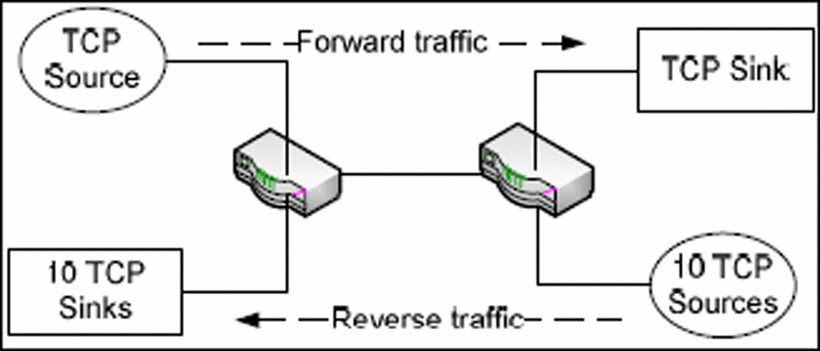
\includegraphics[width=0.5\textwidth]{images/abdeljaouad10_topology_1.png}
	\caption{Figure by I. Abdeljaouad et al.~\cite{Abdeljaouad10}. Topology of the wired ns2 network simulation.}
	\label{fig:topology1}
\end{figure}

\begin{table}
\small
\begin{tabular}{l*{3}{c}l}
& Compound & Cubic & New Reno & Rev. Traffic \\
\hline
0s-250s Mbps & 1.99 & 1.99 & 1.98 & No \\
250s-500s Mbps & 1.79 & 1.96 & 1.71 & Yes \\
500s-750s Mbps & 2.00 & 2.00 & 1.99 & No \\
750s-1000s Mbps & 1.80 & 1.96 & 1.76 & Yes \\
\end{tabular}
\caption{Based on results by I. Abdeljaouad et al.~\cite{Abdeljaouad10}. Goodput achieved by each TCP variant with and without reverse traffic at different time intervals.}
\label{tab:goodput1}
\end{table}

In this scenario, Cubic and Compound were both able to utilize the whole path capacity when no other traffic was present, both performing slightly better than New Reno. When reverse traffic was introduced, Cubic clearly outperformed Compound and New Reno, and Compound performed slightly better than New Reno.  

To measure the fairness of the TCP variants, the set up was slightly modified. Instead of one sender and one sink in the forward path, $M$ sources and sinks were simulated. Figure~\ref{fig:topology2} shows the modified network topology.

\begin{figure}
	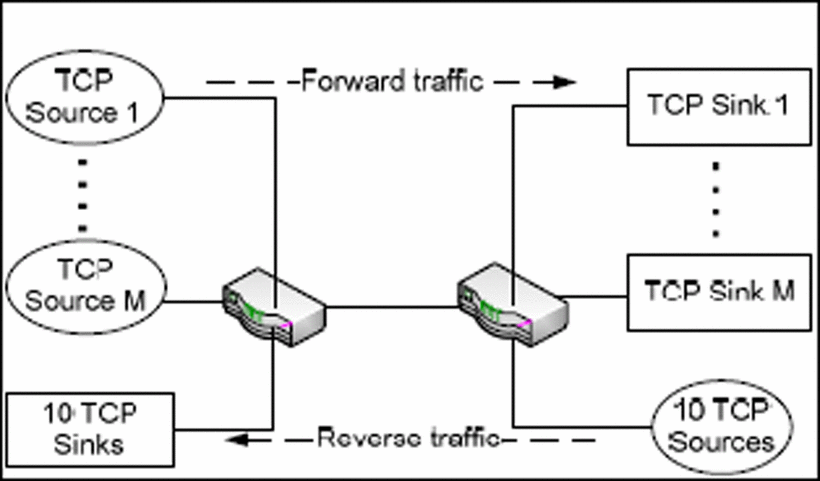
\includegraphics[width=0.5\textwidth]{images/abdeljaouad10_topology_2.png}
	\caption{Figure by I. Abdeljaouad et al.~\cite{Abdeljaouad10}. Topology of the wired ns2 network simulation to measure the fairness of the TCP variants.}
	\label{fig:topology2}
\end{figure}

The fairness was measured for each TCP variant with the number of concurrent senders, $M$, varying from 10 to 200. The RTTs of the senders were randomly selected from a uniform distribution ranging from $20 + 230/M$ to $250$ milliseconds to approximate variance in RTTs of TCP connections in real world. Figure~\ref{fig:fairness1} shows the measured fairness index~\eqref{fairness} for each TCP variant as a function of $M$.

\begin{figure}
	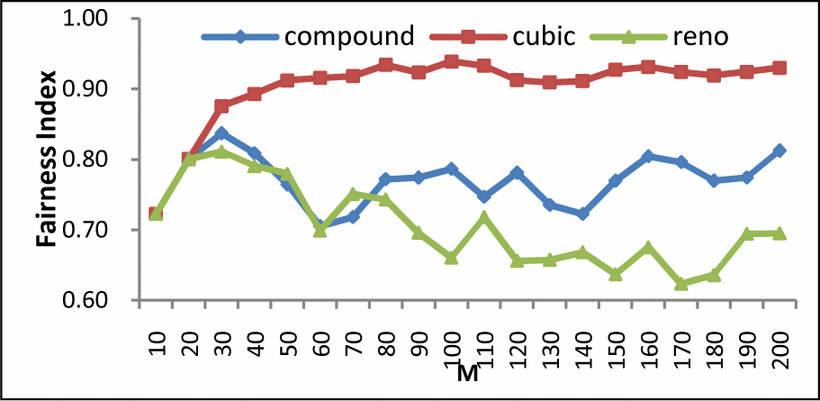
\includegraphics[width=0.5\textwidth]{images/abdeljaouad10_fairness_1.png}
	\caption{Figure by I. Abdeljaouad et al.~\cite{Abdeljaouad10}. Fairness of TCP variants as a function of concurrent senders.}
	\label{fig:fairness1}
\end{figure}

The measurements clearly show that Cubic has the highest fairness of the variants. This result is likely due to the fact that the Cubic treats connections with different RTTs equally, whereas the other variants favour connections with short RTTs. Compound seems to be somewhat fairer than New Reno when the number of concurrent connections is greater than 70. 

In the second set of simulations, the authors looked at the behaviour of the TCP variants over wireless links. The scenario was similar to the previously discussed simulations, except now the TCP sources and sinks at the end of the forward path were mobile and the wireless link was the bottleneck of the connections. All wired links were 1Gbps, while the wireless link and the mobile nodes ran the IEEE802.11g protocol at 54Mbps data rate. Figure~\ref{fig:topology3} shows the network topology of this scenario. Reverse traffic was introduced to the network similarly to the wired scenario.     

\begin{figure}
	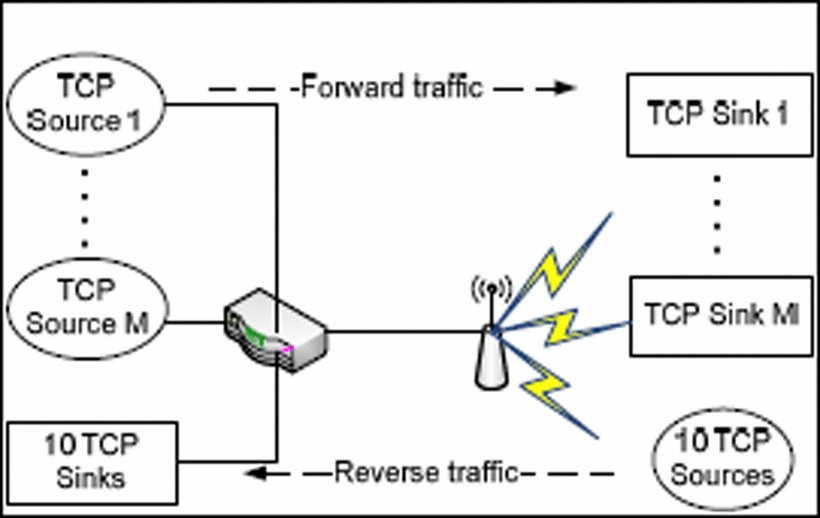
\includegraphics[width=0.5\textwidth]{images/abdeljaouad10_topology_3.png}
	\caption{Figure by I. Abdeljaouad et al.~\cite{Abdeljaouad10}. Topology of the wireless ns2 simulation.}
	\label{fig:topology3}
\end{figure}

The measurements show that New Reno outperformed Compound and Cubic in both goodput and fairness. This is not surprising, since Cubic and Compound are optimized for high throughput networks~\cite{Ha08,Tan05}. The goodputs obtained by all the variants are quite low. The authors argue, that this is mainly due to the reverse traffic causing ACK packages to be drastically delayed, which severely hampers the performance of all three variants. Figure~\ref{fig:goodput} contains the goodputs measured for each variant as a function of concurrent connections.

\begin{figure}
	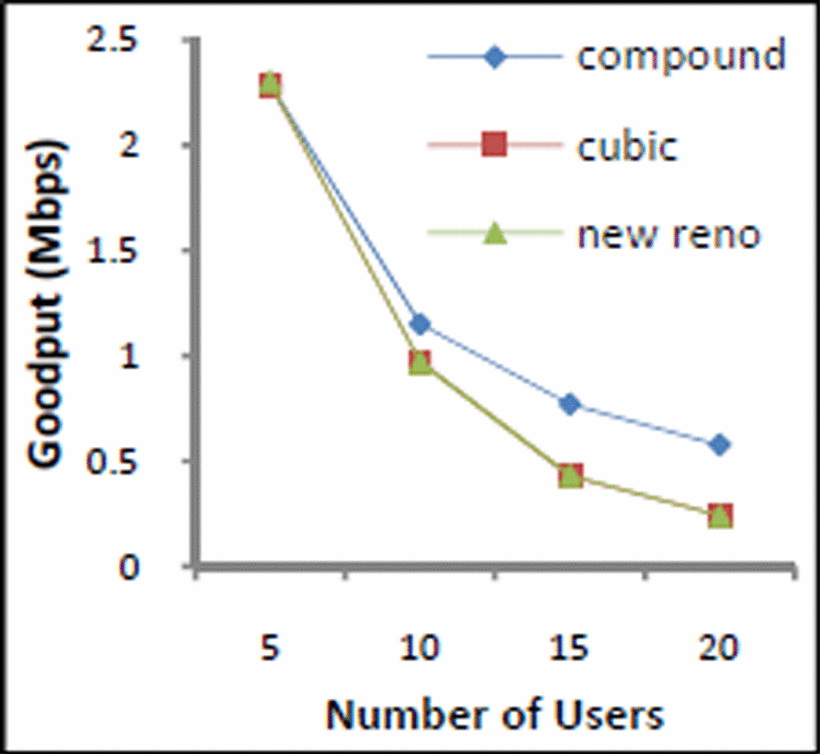
\includegraphics[width=0.5\textwidth]{images/abdeljaouad10_goodput.png}
	\caption{Figure by I. Abdeljaouad et al.~\cite{Abdeljaouad10}. Goodputs obtained by the TCP variants in the wireless ns2 simulation as a function of concurrent connections. }
	\label{fig:goodput}
\end{figure}

All the protocols achieved a good level of fairness in this set up, New Reno being fairest by a clear margin and Cubic performing slightly better than Compound. Figure~\ref{fig:fairness2} contains the fairness~\eqref{fairness} measured for each variant as a function of concurrent connections.

\begin{figure}
	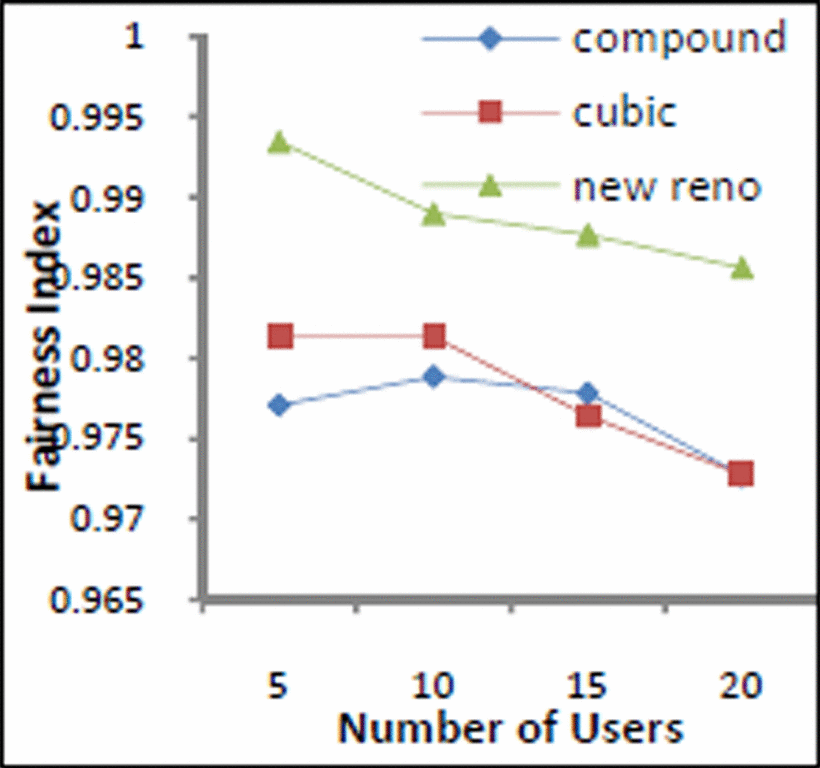
\includegraphics[width=0.5\textwidth]{images/abdeljaouad10_fairness_2.png}
	\caption{Figure by I. Abdeljaouad et al.~\cite{Abdeljaouad10}. Fairness index measured for the TCP variants in the wireless ns2 simulation as a function of concurrent connections.}
	\label{fig:fairness2}
\end{figure}